        %%******************************************%%
        %%                                          %%
        %%        Modello di tesi di laurea         %%
        %%            di Andrea Volpe               %%
        %%                                          %%
        %%             31 ottobre 2022              %%
        %%                                          %%
        %%******************************************%%


% I seguenti commenti speciali impostano:
% 1. 
% 2. PDFLaTeX come motore di composizione;
% 3. tesi.tex come documento principale;
% 4. il controllo ortografico italiano per l'editor.

% !TEX encoding = UTF-8
% !TEX TS-program = pdflatex
% !TEX root = tesi.tex
% !TEX spellcheck = it-IT

% PDF/A filecontents
\RequirePackage{filecontents}
\begin{filecontents*}{\jobname.xmpdata}
  \Title{Migrazione e analisi comparativa di un back-end per un servizio di smart parking}
  \Author{Andrea Volpe}
  \Language{it-IT}
  \Subject{The abstract, or short description.}
  \Keywords{keyword1\sep keyword2\sep keyword3}
\end{filecontents*}

\documentclass[10pt,                    % corpo del font principale
               a4paper,                 % carta A4
               twoside,                 % impagina per fronte-retro
               openright,               % inizio capitoli a destra
               english,                 
               italian,                 
               ]{book}    

%**************************************************************
% Importazione package
%************************************************************** 

\PassOptionsToPackage{dvipsnames}{xcolor} % colori PDF/A

\usepackage{colorprofiles}

\usepackage[a-2b,mathxmp]{pdfx}[2018/12/22]
                                        % configurazione PDF/A
                                        % validare in https://www.pdf-online.com/osa/validate.aspx

%\usepackage{amsmath,amssymb,amsthm}    % matematica

\usepackage[T1]{fontenc}                % codifica dei font:
                                        % NOTA BENE! richiede una distribuzione *completa* di LaTeX
\usepackage{float}
\usepackage[utf8]{inputenc}             % codifica di input; anche [latin1] va bene
                                        % NOTA BENE! va accordata con le preferenze dell'editor

\usepackage[english, italian]{babel}    % per scrivere in italiano e in inglese;
                                        % l'ultima lingua (l'italiano) risulta predefinita

\usepackage{bookmark}                   % segnalibri

\usepackage{caption}                    % didascalie

\usepackage{chngpage,calc}              % centra il frontespizio

\usepackage{csquotes}                   % gestisce automaticamente i caratteri (")

\usepackage{emptypage}                  % pagine vuote senza testatina e piede di pagina

\usepackage{epigraph}			% per epigrafi

\usepackage{eurosym}                    % simbolo dell'euro

%\usepackage{indentfirst}               % rientra il primo paragrafo di ogni sezione

\usepackage{graphicx}                   % immagini

\usepackage{hyperref}                   % collegamenti ipertestuali

\usepackage[binding=5mm]{layaureo}      % margini ottimizzati per l'A4; rilegatura di 5 mm

\usepackage{listings}                   % codici

\usepackage{microtype}                  % microtipografia

\usepackage{mparhack,fixltx2e,relsize}  % finezze tipografiche

\usepackage{nameref}                    % visualizza nome dei riferimenti                                      
\usepackage[font=small]{quoting}        % citazioni

\usepackage{subfig}                     % sottofigure, sottotabelle

\usepackage[italian]{varioref}          % riferimenti completi della pagina

\usepackage{booktabs}                   % tabelle                                       
\usepackage{tabularx}                   % tabelle di larghezza prefissata                                    
\usepackage{longtable}                  % tabelle su più pagine                                        
\usepackage{ltxtable}                   % tabelle su più pagine e adattabili in larghezza

\usepackage[toc, acronym]{glossaries}   % glossario
                                        % per includerlo nel documento bisogna:
                                        % 1. compilare una prima volta tesi.tex;
                                        % 2. eseguire: makeindex -s tesi.ist -t tesi.glg -o tesi.gls tesi.glo
                                        % 3. eseguire: makeindex -s tesi.ist -t tesi.alg -o tesi.acr tesi.acn
                                        % 4. compilare due volte tesi.tex.

\usepackage[backend=biber,style=verbose-ibid,hyperref,backref]{biblatex}
                                        % eccellente pacchetto per la bibliografia; 
                                        % produce uno stile di citazione autore-anno; 
                                        % lo stile "numeric-comp" produce riferimenti numerici
                                        % per includerlo nel documento bisogna:
                                        % 1. compilare una prima volta tesi.tex;
                                        % 2. eseguire: biber tesi
                                        % 3. compilare ancora tesi.tex.

\usepackage{listings}
\usepackage{color}

\definecolor{forestgreen}{RGB}{34,139,34}
\definecolor{orangered}{RGB}{239,134,64}
\definecolor{darkblue}{rgb}{0.0,0.0,0.6}
\definecolor{gray}{rgb}{0.4,0.4,0.4}

\lstdefinestyle{XML} {
    language=XML,
    extendedchars=true, 
    breaklines=true,
    breakatwhitespace=true,
    emph={},
    emphstyle=\color{red},
    basicstyle=\ttfamily,
    columns=fullflexible,
    commentstyle=\color{gray}\upshape,
    morestring=[b]",
    morecomment=[s]{<?}{?>},
    morecomment=[s][\color{forestgreen}]{<!--}{-->},
    keywordstyle=\color{orangered},
    stringstyle=\ttfamily\color{black}\normalfont,
    tagstyle=\color{darkblue}\bf,
    morekeywords={attribute,xmlns,version,type,release},
}

\definecolor{lightgray}{rgb}{.9,.9,.9}
\definecolor{darkgray}{rgb}{.4,.4,.4}
\definecolor{purple}{rgb}{0.65, 0.12, 0.82}

\definecolor{primaryblue}{RGB}{6, 0, 255}
\definecolor{mediumblue}{RGB}{0, 112, 193}
\definecolor{carmine}{RGB}{163, 21, 21}
\definecolor{chestnut}{RGB}{127, 56, 20}
\definecolor{vibrantpurple}{RGB}{175, 0, 219}
\definecolor{midgreen}{RGB}{48, 145, 48}
\definecolor{deepblue}{RGB}{7, 16, 128}

\lstdefinelanguage{JavaScript}{
  keywords={class, constructor, private, readonly, this, async, const, new},
  keywordstyle=\color{primaryblue}\bfseries,
  ndkeywords={await, if, throw, try, catch, return, export},
  ndkeywordstyle=\color{vibrantpurple}\bfseries,
  identifierstyle=\color{black},
  sensitive=false,
  comment=[l]{//},
  morecomment=[s]{/*}{*/},
  commentstyle=\color{midgreen}\ttfamily,
  stringstyle=\color{carmine}\ttfamily,
  % classoffset=2,
  % otherkeywords={Injectable, Controller, ara},
  % morekeywords={Injectable, Controller, ara},
  % keywordstyle=\color{chestnut},
  % classoffset=0,
  morestring=[b]',
  morestring=[b]"
}

\lstset{
  linewidth=14cm
}

\input{tesi-config}                     % file con le impostazioni personali

\begin{document}
%**************************************************************
% Materiale iniziale
%**************************************************************
\frontmatter
\input{inizio-fine/frontespizio}
% !TEX encoding = UTF-8
% !TEX TS-program = pdflatex
% !TEX root = ../Volpe_Andrea.tex

%**************************************************************
% Colophon
%**************************************************************
\clearpage
\phantomsection
\thispagestyle{empty}

\hfill

\vfill

\noindent\myName: \textit{\myTitle,}
\myDegree,
\textcopyright\ \myTime.
\input{inizio-fine/dedica}
% !TEX encoding = UTF-8
% !TEX TS-program = pdflatex
% !TEX root = ../Volpe_Andrea.tex

%**************************************************************
% Sommario
%**************************************************************
\cleardoublepage
\phantomsection
\pdfbookmark{Sommario}{Sommario}
\begingroup
\let\clearpage\relax
\let\cleardoublepage\relax
\let\cleardoublepage\relax

\chapter*{Sommario}

Il presente documento descrive il lavoro svolto durante il periodo di stage, della durata di trecento ore, del
laureando Andrea Volpe presso l'azienda Sync Lab nel periodo che va dal 05/09/2022 al 28/10/2022.
\\\\
Lo scopo dello stage era la realizzazione della migrazione di un \gls{back-end-g} esistente sviluppato in Spring, in un \gls{back-end-g}
scritto in NestJS e la stesura un'analisi comparativa tra le due soluzioni.
\\\\
In questo documento vengono descritte le varie fasi di lavoro effettuate durante lo stage. In particolare si descrive la fase
di analisi e progettazione, ristrutturazione del database, verifica e validazione e infine l'analisi comparativa spiegando
quali sono stati i punti di valutazione che hanno portato a preferire una soluzione rispetto all'altra.

%\vfill
%
%\selectlanguage{english}
%\pdfbookmark{Abstract}{Abstract}
%\chapter*{Abstract}
%
%\selectlanguage{italian}

\endgroup			

\vfill


% !TEX encoding = UTF-8
% !TEX TS-program = pdflatex
% !TEX root = ../Volpe_Andrea.tex

%**************************************************************
% Ringraziamenti
%**************************************************************
\cleardoublepage
\phantomsection
\pdfbookmark{Ringraziamenti}{ringraziamenti}

\begin{flushright}{
	\slshape    
	``Poiché la disperazione era un eccesso che non gli apparteneva, si chinò su quanto era rimasto della sua vita, e riiniziò a prendersene cura, con l’incrollabile tenacia di un giardiniere al lavoro, il mattino dopo il temporale.''} \\ 
	\medskip
    --- Alessandro Baricco
\end{flushright}

\bigskip

\begingroup
\let\clearpage\relax
\let\cleardoublepage\relax
\let\cleardoublepage\relax

\chapter*{Ringraziamenti}

\noindent \textit{Desidero ringraziare con affetto i miei genitori per il sostegno, il grande aiuto e per essermi stati vicini in ogni momento durante gli anni di studio.}\\

\noindent \textit{Ho desiderio di ringraziare poi i miei amici per tutti i bellissimi anni passati insieme e le mille avventure vissute.}\\


\noindent \textit{Vorrei inoltre esprimere la mia gratitudine al Prof. Baldan, relatore della mia tesi, per l'aiuto e il sostegno fornitomi durante la stesura del lavoro.}\\

\noindent \textit{Ringrazio il dott. Daniele Zorzi, tutor aziendale e l'Ingegnere Fabio Pallaro, manager sede Sync Lab, per l'opportunità
	fornitami e il supporto dato durante l'intera attività si stage.}\\


\bigskip

\noindent\textit{\myLocation, \myTime}
\hfill \myName

\endgroup


\input{inizio-fine/indici}
\cleardoublepage

%**************************************************************
% Materiale principale
%**************************************************************
\mainmatter
% !TEX encoding = UTF-8
% !TEX TS-program = pdflatex
% !TEX root = ../Volpe_Andrea.tex

%**************************************************************
\chapter{Introduzione}
\label{cap:introduzione}
%**************************************************************

% Introduzione al contesto applicativo.\\

% \noindent Esempio di utilizzo di un termine nel glossario \\
% \gls{api}. \\

% \noindent Esempio di citazione in linea \\
% \cite{site:agile-manifesto}. \\

% \noindent Esempio di citazione nel pie' di pagina \\
% citazione\footcite{womak:lean-thinking} \\

%**************************************************************
\section{L'azienda}
% //TODO: aggiungere parte normalizzazione
Sync Lab nasce a Napoli nel 2002 come software house ed è rapidamente cresciuta nel
mercato dell’Information and Comunications Tecnology (ICT). 
\\\\
A seguito di una
maturazione delle competenze tecnologiche, metodologiche ed applicative nel dominio
del software, l’azienda è riuscita rapidamente a trasformarsi in \gls{System Integrator}\glsfirstoccur conquistando 
significative fette di mercato nei settori mobile, videosorveglianza e sicurezza
delle infrastrutture informatiche aziendali. 
\\\\
Attualmente, Sync Lab ha più di 150 clienti
diretti e finali, con un organico aziendale di 300 dipendenti distribuiti tra le 6 sedi
dislocate in tutta Italia.
Sync Lab si pone come obiettivo principale quello di supportare il cliente nella realizzazione, 
messa in opera e governance di soluzione \gls{IT}\glsfirstoccur, sia dal punto di vista tecnologico,
sia nel governo del cambiamento organizzativo.

\begin{figure}[H]
    \centering
    \includegraphics[height=2.5cm]{logo-synclab}
    \caption{Logo Sync Lab}
\end{figure}

%**************************************************************
\section{Scelta dell'azienda}
Sono venuto a conoscenza dell'azienda Sync Lab grazie al corso d'ingegneria del
software, dove l'azienda è stata il proponente del mio progetto.
\\\\
Sono venuto a conoscenza della proposta di stage di Sync Lab grazie all'evento stage-it 2022. 
L’evento promosso da Assindustria Venetocentro in collaborazione con l’Università 
di Padova per favorire l’incontro tra aziende con progetti innovativi in ambito \gls{IT} e 
studenti dei corsi di laurea in Informatica, Ingegneria informatica e Statistica.
\\\\


%**************************************************************
\section{Introduzione al progetto}

Il progetto di stage consisteva nella migrazione di un progetto esistente realizzato con il framework
Spring, in un progetto con le stesse funzionalità ma realizzato con il framework NestJS.
\\
Il progetto esistente è composto da un set di
\gls{API}\glsfirstoccur \gls{REST}\glsfirstoccur, che vanno a esporre le funzionalità \gls{CRUD}
di un progetto di Smart Parking. 
\\\\
Il proponente ha deciso di effettuare 
la migrazione per fare un'analisi comparativa tra le due soluzioni
e poter valutare quale delle due meglio si adattasse alle esigenze
del prodotto.
\\\\
Il progetto si chiama Smart Parking e consisteva nella realizzazione di una webapp che si occupasse di gestire un sistema
di controllo parcheggi auto in maniera smart. 
\\
Il sistema va ad interrogare una base di dati contenente
l'informazione inerente allo stato di alcuni sensori di parcheggio, fornendo la visualizzazione
dei posti liberi/occupati all'interno di una mappa.
\\\\
L'idea del progetto nasce per agevolare un utente che vuole usufruire di un posto auto all'interno di 
un parcheggio e non vuole perdere tempo in cerca di un posto libero e nemmeno uscire di casa se i posti auto
sono tutti occupati; infatti la webapp oltre a mostrare su una mappa le piazzole libere/occupate, segnala 
anche la disponibilità di posti auto in un parcheggio; il tutto in tempo reale.
\\\\
Era prevista la realizzazione anche di una sezione dedicata ai manutentori, in modo che potessero monitorare
in tempo reale lo stato dei sensori, facilitando quindi il processo di manutenzione.
\\\\
Il progetto prevedeva la realizzazione di un \gls{front-end}\glsfirstoccur con il framework Angular che interagisse 
con le \gls{API} \gls{REST} da realizzare in questo progetto di 
\gls{back-end}\glsfirstoccur.
\clearpage
\begin{figure}[H]
    \centering
    \includegraphics[height=9cm]{front-end-smart-parking}
    \caption{Front-end Smart Parking}
\end{figure}

%**************************************************************
\section{Problematiche riscontrate}
Durante lo svolgimento del progetto si sono presentate alcune criticità, in parte dovute alla mancanza
di conoscenza delle tecnologie da utilizzate. 
\\
Le problematiche riscontrate:

\begin{itemize}
    \item architettura a microservizi: avevo solo una conoscenza basilare
          della tecnologia grazie al corso d'ingegneria del software ma non
          sufficiente per fare un'analisi di migrazione futura del progetto in un'architettura a microservizi;
    \item framework Spring: la conoscenza di questo framework era completamente assente
        ed era importante averla per poter comprendere con chiarezza il software esistente
        di cui doveva essere effettuata la migrazione;
    \item framework Node.js e NestJS: la conoscenza di questi due framework era completamente
        assente. Conoscerli era di fondamentale importanza per poter implementare il servizio
        di \gls{API} \gls{REST} richiesto;
    \item la quantità di \gls{API} \gls{REST} da migrare era troppo elevata per il tempo a disposizione;
    \item il modello della base dati ha dovuto subire adeguamenti rispetto alla prima versione
        per rappresentare nel modo migliore lo scenario funzionale.
\end{itemize}

%**************************************************************
\section{Soluzione scelta}

E' stato scelto di sviluppare il progetto con un architettura di tipo layered architecture. Questo è uno
degli stili architetturali più utilizzati quando si sviluppa un software monolitico. L'idea dietro a 
questa architettura è che i moduli con funzionalità simili sono organizzati in livelli
orizzontali. Quindi ogni livello svolge uno specifico ruolo nell'applicazione.
\\\\
La layered architecture astrae la visione del sistema nel suo insieme, fornendo dettagli 
sufficienti per comprendere ruoli e le responsabilità dei singoli livelli e le relazioni
che intercorrono tra loro.
\\\\
Un'analisi fatta dal proponente ha rivelato questo tipo di architettura adattarsi molto bene al 
servizio di \gls{API} \gls{REST} da realizzare per questo progetto.
\\
Inoltre molti framework per lo sviluppo di applicativi \gls{back-end} si basano su quest'architettura, compresi
Spring e NestJS, che integrano il pattern controller-service-repository; un pattern
che sfrutta la layered architecture, creando tre diversi livelli di astrazione: 
\begin{itemize}
    \item controller: è il livello più alto ed è l'unico responsabile dell'esposizione delle
        funzionalità, in modo che possano essere consumate da entità esterne;
    \item service: livello centrale, gestisce tutta la business logic;
    \item repository: livello più basso, è responsabile di salvare e recuperare i dati da un
        sistema di persistenza, come un database.
\end{itemize}
\clearpage
\leavevmode\newline
Nell'analisi progettuale è stato scelto l'utilizzo della layered architecture come architettura del progetto,
quindi l'utilizzo di framework che integrassero questo tipo di struttura per sviluppare le applicazioni, come 
Spring e NestJS, è stato quasi obbligatorio.
\leavevmode\newline
\begin{figure}[H]
    \centering
    \includegraphics[height=9cm]{controller-service-repository-pattern}
    \caption{Controller-service-repository pattern}
\end{figure}
\leavevmode\newline
Non era prevista la creazione di un sistema di autenticazione per l'accesso alle \gls{API} \gls{REST}, in quanto 
un altro studente tirocinante stava realizzando questa parte.

%**************************************************************
\section{Descrizione del prodotto ottenuto}

All'inizio dello stage era disponibile un \gls{back-end} contenente le \gls{API} \gls{REST}, sviluppato in Spring, pronto per
poter essere messo in esercizio in ambiente di produzione.
\\
Non potendo migrare l'intero set di \gls{API} \gls{REST}, è stato preventivato di sviluppare
le più importanti, in modo da poter effettuare le operazioni \gls{CRUD}\glsfirstoccur più
comuni.
\\\\
Le \gls{API} \gls{REST} espongono un'interfaccia compatibile con quello che ormai è uno standard per la
comunicazione con servizi di tipo \gls{REST}; ovvero per comunicare con loro è necessario effettuare
delle richieste \gls{HTTP}\glsfirstoccur a degli specifici \gls{endpoint} tramite i seguenti metodi:
\begin{itemize}
    \item GET: per ottenere delle risorse dal servizio \gls{REST};
    \item POST: per creare una nuova risorsa nel servizio \gls{REST};
    \item PUT: per modificare una risorsa nel servizio \gls{REST};
    \item DELETE: per eliminare una risorsa dal servizio \gls{REST}.
\end{itemize}
\leavevmode\newline
Nel \gls{back-end} è presente inoltre un servizio schedulato che ogni due minuti in maniera autonoma va a fare il polling
da un file \gls{XML}\glsfirstoccur online, contenente gli stati aggiornati dei sensori. Questo servizio registra poi 
le variazioni, rispetto
al polling precedente, nello strato di persistenza.
\\\\
Il file \gls{XML} viene scritto e gestito dai produttori dei sensori di parcheggio, quindi non era compito di questo 
progetto gestirne il funzionamento. Il funzionamento di questo file \gls{XML} è comunque abbastanza banale,
in quanto ad ogni variazione di stato, il sensore di parcheggio va semplicemente ad aggiornare 
il record a lui associato
all'interno del file.
\\
\begin{figure}[H]
    \centering
    \includegraphics[height=8cm]{polling-sensori}
    \caption{Polling sensori}
\end{figure}
\leavevmode\newline
%**************************************************************
\section{Tecnologie utilizzate}

\textbf{Git}
\\\\
E' uno degli strumenti di controllo di versionamento più utilizzati. Facilita la collaborazione
tra gli sviluppatori nella realizzazione di un progetto e permette con semplicità di spostarsi
tra varie versioni del software realizzate. Nel progetto è stato utilizzato con il workflow
Gitflow.
\\\\\\
\textbf{Visual Studio Code}
\\\\
E' un editor di codice sorgente sviluppato da Microsoft che aiuta lo sviluppatore durante la fase
di sviluppo del codice in quanto evidenzia le parole chiave, segnala errori di scrittura, suggerisce
snippet di codice. Possiede una grande libreria di estensioni facilmente installabili per renderlo
compatibile con praticamente qualsiasi linguaggio di programmazione.
\\\\\\
\textbf{Postman}
\\\\
E' un'applicazione che viene utilizzata solitamente per testare \gls{API}. E' un client \gls{HTTP} che testa richieste
\gls{HTTP} utilizzando una \gls{GUI}\glsfirstoccur, attraverso la quale otteniamo diversi tipi di risposta in base alle \gls{API} che 
andiamo ad interrogare.
\\\\\\
\clearpage
\leavevmode\newline
\textbf{Stoplight}
\\\\
E' una piattaforma per progettare \gls{API}. Grazie a questo strumento è possibile documentare in maniera rigorosa
e su uno spazio in cloud un set di \gls{API}. La piattaforma permette di specificare varie informazioni per ogni
\gls{API}, tra cui \gls{endpoint}\glsfirstoccur, parametri in ingresso attesi, possibili risposte con status code associato. Questo
strumento è molto utile per gli sviluppatori \gls{front-end} che devono chiamare le \gls{API} di un servizio
\gls{back-end}, soprattutto grazie alla funzionalità che permette di generare il \gls{mock}\glsfirstoccur della risposta di un'\gls{API}, 
permettendo allo sviluppatore di effettuare le chiamate al \gls{back-end} anche senza che questo sia stato ancora realizzato.
\\\\\\
\textbf{TypeScript}
\\\\
E' un superset di JavaScript, che aggiunge tipi, classi, interfacce e moduli opzionali al JavaScript 
tradizionale. Si tratta sostanzialmente di una estensione di JavaScript.
TypeScript è un linguaggio tipizzato, ovvero aggiunge definizioni di tipo statico: i tipi consentono di 
descrivere la forma di un oggetto, documentandolo meglio e consentendo a TypeScript di verificare che 
il codice funzioni correttamente.
\\\\\\
\textbf{Node.js}
\\\\
E' un runtime system open source per eseguire applicazioni scritte in JavaScript, permettendoci di utilizzare questo 
linguaggio, tipicamente utilizzato nella client-side, anche per la scrittura di applicazioni server-side.
La piattaforma è basata sul JavaScript Engine V8, che è il runtime di Google utilizzato anche da Chrome e 
disponibile sulle principali piattaforme, anche se maggiormente performante su sistemi operativi UNIX-like.
\\\\\\
\textbf{NestJS}
\\\\
E' un framework per la creazione di applicazioni lato server Node.js efficienti e scalabili. 
Utilizza JavaScript ma è costruito con e supporta completamente TypeScript. Aggiunge un livello di astrazione
al framework Express, che a sua volta aggiunge astrazione al framework Node.js. Di conseguenza NestJS 
utilizza Node.js per eseguire il codice JavaScript generato dalla compilazione del codice TypeScript.
\\\\\\
\textbf{Spring}
\\\\
Spring è un framework leggero, basato su Java. Questo framework integra soluzioni a vari problemi tecnici
che si presentano con alta frequenza durante lo sviluppo software. Spring si basa su due design pattern
fondamentali che sono l'Inversion of Control e Dependency Injection.
\\\\\\
\clearpage
\leavevmode\newline
\textbf{PostgreSQL}
\\\\
Chiamato anche Postgres, è un sistema di database relazionale a oggetti (ORDBMS), open source e 
gratuito.
Le principali caratteristiche di Postgres sono affidabilità, integrità dei dati, funzionalità ed estensibilità, 
oltre alla propria community open source che gestisce, aggiorna e sviluppa soluzioni performanti e innovative.
\\\\\\
\textbf{Jest}
\\\\
Jest è un framework di unit test sviluppato da Facebook. Focalizzato sulla semplicità, è utilizzabile in qualsiasi
progetto JavaScript. E'uno dei framework di test JavaScript più popolare in questi giorni e la scelta di default 
per alcuni framework come NestJS e React.
\\\\\\
\textbf{Winston}
\\\\
Winston è una delle libreria più famose per effettuare il logging su applicazioni Node.js. Permette di effettuare il logging
su più livelli di informazione, formattare il logging in modo predefinito, scegliere la destinazione di output del log e molte 
altre opzioni.
\\\\\\
\textbf{Npm}
\\\\
E' uno dei gestori di pacchetti per il linguaggio JavaScript più popolare. E' il gestore di pacchetti predefinito 
per Node.js.

%**************************************************************
\section{Organizzazione del testo}

\begin{description}
    \item[{\hyperref[cap:analisi-requisiti]{Il secondo capitolo}}] descrive l'analisi dei requisiti.
    
    \item[{\hyperref[cap:progettazione]{Il terzo capitolo}}] approfondisce la fase di progettazione.
    
    \item[{\hyperref[cap:ristrutturazione-database]{Il quarto capitolo}}] descrive la fase di ristrutturazione del database.
    
    \item[{\hyperref[cap:verifica-e-validazione]{Il quinto capitolo}}] descrive la fase di verifica e validazione.
    
    \item[{\hyperref[cap:analisi-comparativa]{Il sesto capitolo}}] approfondisce l'analisi comparativa tra la soluzione in Spring e quella in NestJS.
    
    \item[{\hyperref[cap:conclusioni]{Il settimo capitolo}}] presenta le conclusioni finali sul progetto e sull'esperienza di stage.
\end{description}

Riguardo la stesura del testo, relativamente al documento sono state adottate le seguenti convenzioni tipografiche:
\begin{itemize}
	\item gli acronimi, le abbreviazioni e i termini ambigui o di uso non comune menzionati vengono definiti nel glossario, situato alla fine del presente documento;
	\item per la prima occorrenza dei termini riportati nel glossario viene utilizzata la seguente nomenclatura: \emph{parola}\glsfirstoccur.
\end{itemize}             % Introduzione
% !TEX encoding = UTF-8
% !TEX TS-program = pdflatex
% !TEX root = ../tesi.tex

%**************************************************************
\chapter{Analisi dei requisiti}
\label{cap:analisi-requisiti}
%**************************************************************

\section{Confronto con gli stakeholders}
E' stato fatto un incontro iniziale con il proponente, ovvero l'azienda Sync Lab,
per definire con chiarezza i requisiti richiesti.
\\\\
Nell'incontro sono state prese in considerazione le REST API scritte col framework Spring 
già esistenti di cui doveva esserne fatta la migrazione nel framework NestJS.
E' emerso subito che la quantità di REST API da realizzare era troppo elevata per la
quantità di tempo a disposizione. 
\\\\
E' stato quindi necessario fare una valutazione di quali fossero i servizi fondamentali che
il servizio di REST API avrebbe dovuto esporre, per poter essere utilizzato senza che venissero
a mancare funzionalità fondamentali per l'utilizzo a livello base del sistema.
\\\\
Ho realizzato quindi un elenco di casi d'uso, in approvazione con la proponente, per avere più
chiari i requisiti del progetto.

\section{Entità}
Per rendere più chiaro il dominio del progetto ed eliminare eventuali ambiguità è stato necessario
documentare le entità di dominio, coinvolte nelle funzionalità fondamentali delle REST API, di cui si
è deciso effettuare la migrazione.
\\\\
Piazzola
\\
Modella il rettangolo bianco dipinto sull'asfalto che delimita la zona in cui l'automobile viene messa
in sosta. Ogni piazzola deve essere associata ad un parcheggio. Una piazzola può avere un solo sensore
di parcheggio.
\\
Ogni piazzola è caratterizzata da:
\begin{itemize}
    \item id: numero incrementale.
    \item latitudine: stringa.
    \item longitudine: stringa.
\end{itemize}
\leavevmode\newline
Parcheggio
\\
Modella l'insieme di piazzole.
\\
Ogni parcheggio è caratterizzato da:
\begin{itemize}
    \item id: numero incrementale.
    \item latitudine: stringa.
    \item longitudine: stringa.
\end{itemize}
\leavevmode\newline
Sensore
\\
Modella il sensore. Esistono due tipi di sensore:
\begin{itemize}
    \item ambientale: misurano la qualità dell'aria e altri parametri nel parcheggio e possono 
        coprire un'area di N piazzole.
        Sono gestiti da un'altro progetto di tirocinio, quindi non sono facenti parte di questo dominio di progetto.
    \item di parcheggio: sensore posizionato sotto l'auto nella piazzola, che rileva la presenza o meno
        del veicolo. Questo tipo di sensore può essere associato a una sola piazzola.
\end{itemize}
Ogni sensore può avere una sola azienda manutentrice a lui associata.
Ogni sensore è caratterizzato da:
\begin{itemize}
    \item id: numero incrementale.
    \item nome: stringa.
    \item batteria: stringa, indica la tensione della batteria in Volt.
    \item carica: stringa, indica il livello di carica della batteria (da 1 a 3).
    \item type: stringa, indica il tipo di sensore (ambientale o di parcheggio).
    \item attivo: booleano.
    \item ultimo sondaggio: data, indica l'ultima volta che è stato aggiornato lo stato del sensore.
    \item da riparare: booleano, indica se il sensore deve essere riparato.
    \item da caricare: booleano, indica se la batteria del sensore è scarica.
    \item in aggiornamento: booleano, indica se il sensore stà aggiornando il suo software.
\end{itemize}
\leavevmode\newline
Manutentore
\\
Modella l'azienda incaricata alla manutenzione dei sensori.
Ogni manutentore è caratterizzato da:
\begin{itemize}
    \item id: numero incrementale.
    \item nome: stringa, indica il nome del titolare dell'azienda.
    \item cognome: stringa, indica il cognome del titolare dell'azienda.
    \item azienda: stringa.
    \item telefono: stringa.
    \item email: stringa.
\end{itemize}
\leavevmode\newline
Misurazione sensore parcheggio.
\\
Modella la misurazione effettuata dal sensore di parcheggio. A differenza di un sensore ambientale, un sensore
di parcheggio non salva uno storico di misurazioni fatte ma viene inserita solo l'ultima misurazione effettuata,
sovrascrivendo la precedente.
Ogni misurazione di un sensore di parcheggio è caratterizzata da:
\begin{itemize}
    \item id: numero incrementale.
    \item indirizzo: stringa.
    \item latitudine: stringa.
    \item longitudine: stringa.
    \item valore: booleano, indica se il veicolo è presente o meno sopra al sensore.
    \item marca temporale: data, indica la data in cui è stata effettuata la misurazione.
\end{itemize}

\section{Casi d'uso}
Definite le entità di dominio si è proceduto con la creazione dei casi d'uso.
\\
Per maggior chiarezza i casi d'uso sono stati raggruppati per entità di dominio di appartenenza.
\\\\

% parcheggio
\begin{figure}[!h]
    \centering
    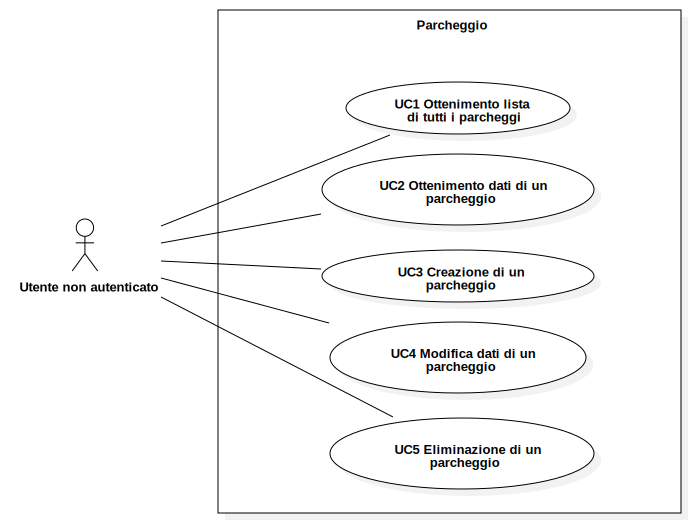
\includegraphics[height=9cm]{usecase/parking-area}
\end{figure}
UC1 - Ottenimento lista di tutti i parcheggi.
\\
Attori primari: utente non autenticato.
\\
Precondizioni: l'utente è in possesso degli strumenti per poter effettuare la richiesta al sistema.
\\
Post-condizioni: l'utente ha ottenuto una lista di tutti i parcheggi.
\\
Scenario principale:
\begin{enumerate}
    \item l'utente richiede la lista di tutti i parcheggi.
    \item l'utente ottiene una lista di tutti i parcheggi.
\end{enumerate}
\leavevmode\newline
UC2 - Ottenimento dati di un parcheggio.
\\
Attori primari: utente non autenticato.
\\
Precondizioni: l'utente è in possesso degli strumenti per poter effettuare la richiesta al sistema.
\\
Post-condizioni: l'utente ha ottenuto i dati di un parcheggio.
\\
Scenario principale:
\begin{enumerate}
    \item l'utente richiede i dati di un parcheggio.
    \item l'utente ottiene i dati di un parcheggio.
\end{enumerate}
\leavevmode\newline
UC3 - Creazione di un parcheggio.
\\
Attori primari: utente non autenticato.
\\
Precondizioni: l'utente è in possesso degli strumenti per poter effettuare la richiesta al sistema.
\\
Post-condizioni: l'utente ha creato un parcheggio.
\\
Scenario principale:
\begin{enumerate}
    \item l'utente richiede la creazione di un parcheggio.
    \item l'utente crea un parcheggio.
\end{enumerate}
\leavevmode\newline
UC4 - Modifica dati di un parcheggio.
\\
Attori primari: utente non autenticato.
\\
Precondizioni: l'utente è in possesso degli strumenti per poter effettuare la richiesta al sistema.
\\
Post-condizioni: l'utente ha modificato un parcheggio.
\\
Scenario principale:
\begin{enumerate}
    \item l'utente richiede la modifica di un parcheggio.
    \item l'utente modifica un parcheggio.
\end{enumerate}
\leavevmode\newline
UC5 - Eliminazione di un parcheggio.
\\
Attori primari: utente non autenticato.
\\
Precondizioni: l'utente è in possesso degli strumenti per poter effettuare la richiesta al sistema.
\\
Post-condizioni: l'utente ha eliminato un parcheggio.
\\
Scenario principale:
\begin{enumerate}
    \item l'utente richiede l'eliminazione di un parcheggio.
    \item l'utente elimina un parcheggio.
\end{enumerate}

% manutentore
\leavevmode\newline

\begin{figure}[!h]
    \centering
    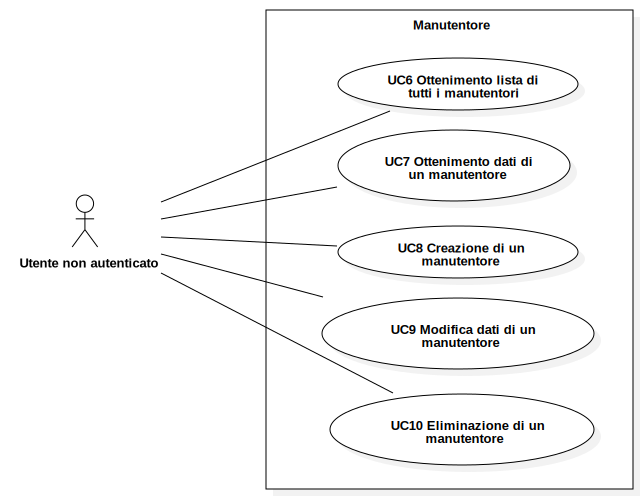
\includegraphics[height=9cm]{usecase/maintainer}
\end{figure}
UC6 - Ottenimento lista di tutti i manutentori.
\\
Attori primari: utente non autenticato.
\\
Precondizioni: l'utente è in possesso degli strumenti per poter effettuare la richiesta al sistema.
\\
Post-condizioni: l'utente ha ottenuto una lista di tutti i manutentori.
\\
Scenario principale:
\begin{enumerate}
    \item l'utente richiede la lista di tutti i manutentori.
    \item l'utente ottiene una lista di tutti i manutentori.
\end{enumerate}
\leavevmode\newline
UC7 - Ottenimento dati di un manutentore.
\\
Attori primari: utente non autenticato.
\\
Precondizioni: l'utente è in possesso degli strumenti per poter effettuare la richiesta al sistema.
\\
Post-condizioni: l'utente ha ottenuto i dati di un manutentore.
\\
Scenario principale:
\begin{enumerate}
    \item l'utente richiede i dati di un manutentore.
    \item l'utente ottiene i dati di un manutentore.
\end{enumerate}
\leavevmode\newline
UC8 - Creazione di un manutentore.
\\
Attori primari: utente non autenticato.
\\
Precondizioni: l'utente è in possesso degli strumenti per poter effettuare la richiesta al sistema.
\\
Post-condizioni: l'utente ha creato un manutentore.
\\
Scenario principale:
\begin{enumerate}
    \item l'utente richiede la creazione di un manutentore.
    \item l'utente crea un manutentore.
\end{enumerate}
\leavevmode\newline
UC9 - Modifica dati di un manutentore.
\\
Attori primari: utente non autenticato.
\\
Precondizioni: l'utente è in possesso degli strumenti per poter effettuare la richiesta al sistema.
\\
Post-condizioni: l'utente ha modificato un manutentore.
\\
Scenario principale:
\begin{enumerate}
    \item l'utente richiede la modifica di un manutentore.
    \item l'utente modifica un manutentore.
\end{enumerate}
\leavevmode\newline
UC10 - Eliminazione di un manutentore.
\\
Attori primari: utente non autenticato.
\\
Precondizioni: l'utente è in possesso degli strumenti per poter effettuare la richiesta al sistema.
\\
Post-condizioni: l'utente ha eliminato un manutentore.
\\
Scenario principale:
\begin{enumerate}
    \item l'utente richiede l'eliminazione di un manutentore.
    \item l'utente elimina un manutentore.
\end{enumerate}

% sensore
\leavevmode\newline
\begin{figure}[!h]
    \centering
    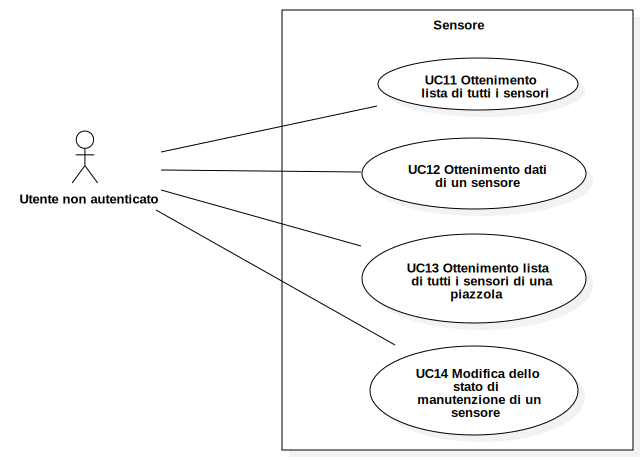
\includegraphics[height=9cm]{usecase/sensor}
\end{figure}
UC11 - Ottenimento lista di tutti i sensori.
\\
Attori primari: utente non autenticato.
\\
Precondizioni: l'utente è in possesso degli strumenti per poter effettuare la richiesta al sistema.
\\
Post-condizioni: l'utente ha ottenuto una lista di tutti i sensori.
\\
Scenario principale:
\begin{enumerate}
    \item l'utente richiede la lista di tutti i sensori.
    \item l'utente ottiene una lista di tutti i sensori.
\end{enumerate}
\leavevmode\newline
UC12 - Ottenimento dati di un sensore.
\\
Attori primari: utente non autenticato.
\\
Precondizioni: l'utente è in possesso degli strumenti per poter effettuare la richiesta al sistema.
\\
Post-condizioni: l'utente ha ottenuto i dati di un sensore.
\\
Scenario principale:
\begin{enumerate}
    \item l'utente richiede i dati di un sensore.
    \item l'utente ottiene i dati di un sensore.
\end{enumerate}
\leavevmode\newline
UC13 - Ottenimento lista di tutti i sensori di una piazzola.
\\
Attori primari: utente non autenticato.
\\
Precondizioni: l'utente è in possesso degli strumenti per poter effettuare la richiesta al sistema.
\\
Post-condizioni: l'utente ha ottenuto una lista di tutti i sensori di una piazzola.
\\
Scenario principale:
\begin{enumerate}
    \item l'utente richiede la lista di tutti i sensori di una piazzola.
    \item l'utente ottiene una lista di tutti i sensori di una piazzola.
\end{enumerate}
\leavevmode\newline
UC14 - Modifica dello stato di manutenzione di un sensore.
\\
Attori primari: utente non autenticato.
\\
Precondizioni: l'utente è in possesso degli strumenti per poter effettuare la richiesta al sistema.
\\
Post-condizioni: l'utente ha modificato lo stato di manutenzione di un sensore.
\\
Scenario principale:
\begin{enumerate}
    \item l'utente richiede la modifica dello stato di manutenzione di un sensore.
    \item l'utente modifica lo stato di manutenzione di un sensore.
\end{enumerate}

% piazzola
\leavevmode\newline
\begin{figure}[!h]
    \centering
    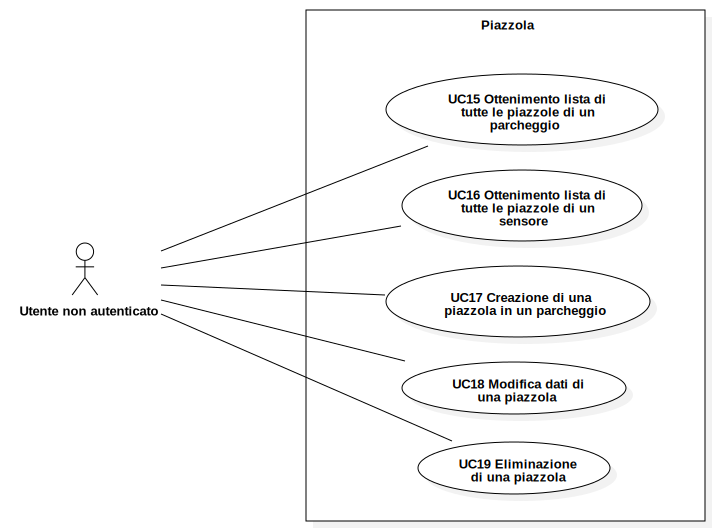
\includegraphics[height=9cm]{usecase/parking-spot}
\end{figure}
UC15 - Ottenimento lista di tutte le piazzole di un parcheggio.
\\
Attori primari: utente non autenticato.
\\
Precondizioni: l'utente è in possesso degli strumenti per poter effettuare la richiesta al sistema.
\\
Post-condizioni: l'utente ha ottenuto una lista di tutte le piazzole di un parcheggio.
\\
Scenario principale:
\begin{enumerate}
    \item l'utente richiede la lista di tutte le piazzole di un parcheggio.
    \item l'utente ottiene una lista di tutte le piazzole di un parcheggio.
\end{enumerate}
\leavevmode\newline
UC16 - Ottenimento lista di tutte le piazzole di un sensore.
\\
Attori primari: utente non autenticato.
\\
Precondizioni: l'utente è in possesso degli strumenti per poter effettuare la richiesta al sistema.
\\
Post-condizioni: l'utente ha ottenuto una lista di tutte le piazzole di un sensore.
\\
Scenario principale:
\begin{enumerate}
    \item l'utente richiede la lista di tutte le piazzole di un sensore.
    \item l'utente ottiene una lista di tutte le piazzole di un sensore.
\end{enumerate}
\leavevmode\newline
UC17 - Creazione di una piazzola in un parcheggio.
\\
Attori primari: utente non autenticato.
\\
Precondizioni: l'utente è in possesso degli strumenti per poter effettuare la richiesta al sistema.
\\
Post-condizioni: l'utente ha creato una piazzola in un parcheggio.
\\
Scenario principale:
\begin{enumerate}
    \item l'utente richiede la creazione di una piazzola in un parcheggio.
    \item l'utente crea una piazzola in un parcheggio.
\end{enumerate}
\leavevmode\newline
UC18 - Modifica dati di una piazzola.
\\
Attori primari: utente non autenticato.
\\
Precondizioni: l'utente è in possesso degli strumenti per poter effettuare la richiesta al sistema.
\\
Post-condizioni: l'utente ha modificato una piazzola.
\\
Scenario principale:
\begin{enumerate}
    \item l'utente richiede la modifica di una piazzola.
    \item l'utente modifica una piazzola.
\end{enumerate}
\leavevmode\newline
UC19 - Eliminazione di una piazzola.
\\
Attori primari: utente non autenticato.
\\
Precondizioni: l'utente è in possesso degli strumenti per poter effettuare la richiesta al sistema.
\\
Post-condizioni: l'utente ha eliminato una piazzola.
\\
Scenario principale:
\begin{enumerate}
    \item l'utente richiede l'eliminazione di una piazzola.
    \item l'utente elimina una piazzola.
\end{enumerate}

% misurazione
\leavevmode\newline
\begin{figure}[!h]
    \centering
    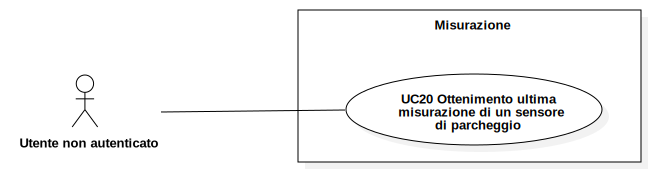
\includegraphics[height=9cm]{usecase/parking-sensor}
\end{figure}
UC20 - Ottenimento ultima misurazione di un sensore di parcheggio.
\\
Attori primari: utente non autenticato.
\\
Precondizioni: l'utente è in possesso degli strumenti per poter effettuare la richiesta al sistema.
\\
Post-condizioni: l'utente ha ottenuto l'ultima misurazione di un sensore di parcheggio.
\\
Scenario principale:
\begin{enumerate}
    \item l'utente richiede l'ultima misurazione di un sensore di parcheggio.
    \item l'utente ottiene l'ultima misurazione di un sensore di parcheggio.
\end{enumerate}

% TODO: inserire sotto casi d'uso specificando i campi da visualizzare / modificare
\section{Tracciamento dei requisiti}
Ogni requisito è identificato da un codice univoco nel seguente formato:
\begin{itemize}
    \item la prima lettera è sempre R, a indicare la parola requisito
    \item la seconda lettera indica il tipo di requisito:
    \begin{itemize}
        \item F per i requisiti funzionali
        \item Q per i requisiti qualitativi
        \item V per i requisiti di vincolo
    \end{itemize}
    \item un numero progressivo che identifica in modo univoco il requisito.
\end{itemize}
Per maggior chiarezza i requisiti sono stati raggruppati per entità di dominio di appartenenza.

% parcheggio
\leavevmode\newline
\begin{table}
    \begin{tabular}{|p{1cm}|p{6cm}|p{1.9cm}|p{1cm}|} 
    \hline
    Codice & Descrizione & Rilevanza &  Fonti \\ 
    \hline
    RF1 & L'utente non autenticato deve poter ottenere la lista di tutti i parcheggi. & Obbligatorio & UC1 \\ 
    \hline
    RF2 & L'utente non autenticato deve poter ottenere i dati di un parcheggio. & Obbligatorio & UC2 \\ 
    \hline
    RF3 & L'utente non autenticato deve poter creare un parcheggio. & Obbligatorio & UC3 \\ 
    \hline
    RF4 & L'utente non autenticato deve poter modificare i dati di un parcheggio. & Obbligatorio & UC4 \\
    \hline
    RF5 & L'utente non autenticato deve poter eliminare un parcheggio. & Obbligatorio & UC5 \\ 
    \hline
    \end{tabular}
\end{table}

% manutentore
\leavevmode\newline
\begin{table}
    \begin{tabular}{|p{1cm}|p{6cm}|p{1.9cm}|p{1cm}|} 
    \hline
    Codice & Descrizione & Rilevanza &  Fonti \\ 
    \hline
    RF6 & L'utente non autenticato deve poter ottenere la lista di tutti i manutentori. & Obbligatorio & UC6 \\ 
    \hline
    RF7 & L'utente non autenticato deve poter ottenere i dati di un manutentore. & Obbligatorio & UC7 \\ 
    \hline
    RF8 & L'utente non autenticato deve poter creare un manutentore. & Obbligatorio & UC8 \\ 
    \hline
    RF9 & L'utente non autenticato deve poter modificare i dati di un manutentore. & Obbligatorio & UC9 \\
    \hline
    RF10 & L'utente non autenticato deve poter eliminare un manutentore. & Obbligatorio & UC10 \\ 
    \hline
    \end{tabular}
\end{table}

% sensore
\leavevmode\newline
\begin{table}
    \begin{tabular}{|p{1cm}|p{6cm}|p{1.9cm}|p{1cm}|} 
    \hline
    Codice & Descrizione & Rilevanza &  Fonti \\ 
    \hline
    RF11 & L'utente non autenticato deve poter ottenere la lista di tutti i sensori. & Obbligatorio & UC11 \\ 
    \hline
    RF12 & L'utente non autenticato deve poter ottenere i dati di un sensori. & Obbligatorio & UC12 \\ 
    \hline
    RF13 & L'utente non autenticato deve poter ottenere la lista di tutti i sensori di una piazzola. & Obbligatorio & UC13 \\ 
    \hline
    RF14 & L'utente non autenticato deve poter modificare lo stato di manutenzione di un sensore. & Obbligatorio & UC14 \\ 
    \hline
    \end{tabular}
\end{table}

% piazzola
\leavevmode\newline
\begin{table}
    \begin{tabular}{|p{1cm}|p{6cm}|p{1.9cm}|p{1cm}|} 
    \hline
    Codice & Descrizione & Rilevanza &  Fonti \\ 
    \hline
    RF15 & L'utente non autenticato deve poter ottenere la lista di tutte le piazzole di un parcheggio. & Obbligatorio & UC15 \\ 
    \hline
    RF16 & L'utente non autenticato deve poter ottenere la lista di tutte le piazzole di un sensore. & Obbligatorio & UC16 \\ 
    \hline
    RF17 & L'utente non autenticato deve poter creare una piazzola in un parcheggio. & Obbligatorio & UC17 \\ 
    \hline
    RF18 & L'utente non autenticato deve poter modificare i dati di una piazzola. & Obbligatorio & UC18 \\
    \hline
    RF19 & L'utente non autenticato deve poter eliminare una piazzola. & Obbligatorio & UC19 \\
    \hline
    \end{tabular}
\end{table}

% misurazione
\leavevmode\newline
\begin{table}
    \begin{tabular}{|p{1cm}|p{6cm}|p{1.9cm}|p{1cm}|} 
    \hline
    Codice & Descrizione & Rilevanza &  Fonti \\ 
    \hline
    RF20 & L'utente non autenticato deve poter ottenere l'ultima misurazione di un sensore di parcheggio. & Obbligatorio & UC20 \\ 
    \hline
    \end{tabular}
\end{table}

% TODO: aggiungere requisiti facoltativi e desiderabili. Aggiungere requisiti qualitativi e di vincolo.             % Processi
% !TEX encoding = UTF-8
% !TEX TS-program = pdflatex
% !TEX root = ../tesi.tex

%**************************************************************
\chapter{Progettazione}
\label{cap:progettazione}
%**************************************************************

% \intro{Breve introduzione al capitolo}\\

% %**************************************************************
\section{Architettura del progetto}
Dato le dimensioni contenute del progetto e per il fatto che deve essere fatta un'analisi 
comparativa con un'altro progetto, si è deciso di strutturarlo con un'architettura a monolite
basata sulla layered architecture.
\\
In questo modo viene velocizzata la realizzazione del progetto, a discapito della facilità di
manutenzione ma non è un problema essendo questo progetto di dimensioni contenute ed in caso
il progetto dovesse crescere fino al punto in cui risulti difficile manutenerlo è sempre possibile
migrarlo in un progetto con un'architettura a microservizi.

% ref: https://cs.uwaterloo.ca/~m2nagapp/courses/CS446/1195/Arch_Design_Activity/Layered.pdf
\subsection{Layered architecture}
La layered architecture è uno degli stili architetturali più utilizzati. L'idea che sta dietro a
questo tipo di architettura è che i moduli o i componenti con funzionalità simili sono organizzati
in livelli orizzontali. Di conseguenza ogni livello svolge un ruolo specifico nell'applicazione.
\\
La layered architecture non ha restrizioni sul numero di strati che l'applicazione può avere, in quanto 
lo scopo è avere livelli che promuovano il concetto di separazione delle responsabilità.
\begin{figure}[!h]
    \centering
    \includegraphics[height=6cm]{layered-architecture}
\end{figure}
\leavevmode\newline
Solitamente ogni livello comunica solo con il livello sottostante. Il connettore tra ogni livello può 
essere una chiamata di funzione, una richiesta di query, un oggetto dati o qualsiasi connettore che
trasmetta richieste o informazioni.
\\
La denominazione dei livelli è abbastanza flessibile ma di solito un livello di presentazione, un livello
di business e un livello fisico sono sempre presenti
\\\\
Livello di presentazione
\\
Il livello di presentazione contiene tutte le classi responsabili di presentare la visualizzazione delle
delle informazioni all'utente finale. Idealmente questo è il solo livello con cui l'utente finale 
interagisce.
\\\\
Livello di business
\\
Il livello di business contiene tutta la logica che è richiesta dall'applicazione per poter soddisfare i 
suoi requisiti funzionali. Solitamente questo livello si occupa dell'aggregazione dei dati, della computazione
e della richiesta dei dati. Quindi qui è dove viene implementata la logica principale dell'applicazione.
\\\\
Livello fisico
\\
Qui è dove sono salvati tutti i dati recuperabili dell'applicazione. Solitamente questo livello è chiamato
anche livello di persistenza. Questo livello si occupa di interagire con il sistema in cui i dati 
sono mantenuti in maniera persistente, come ad esempio un database.
\leavevmode\newline
\subsection{Motivazioni della scelta}
Le motivazione che hanno portato a scegliere questo stile architetturale sono le seguenti:
\begin{itemize}
    \item Dato che la separazione delle responsabilità è la proprietà principale di quest'architettura,
        ogni livello di software ha la sua specifica funzione. Questo rende facile il dover aggiornare 
        singoli livelli e permette al team di sviluppo di separare bene i carichi di lavoro tra i vari 
        membri, che possono lavorare in maniera contemporanea su livelli diversi.
    \item Per la proponente è importante avere una suite di test automatici per testare i vari componenti
        dell'applicazione. La layered architecture separando bene le responsabilità tra i livelli, 
        permette di suddividere l'applicazione in componenti ben separati e quindi più facili da testare.
        Essendo ogni livello isolato dagli altri, è possibile creare casi di test di dimensione ridotta, 
        in quanto le componenti di cui fare il mock sono poche.
    \item L'isolamento tra i vari livelli permette di modificare un livello senza che la modifica intacchi
        gli altri livelli.
    \item Nel caso l'applicazione diventi molto grande è possibile senza troppo sforzo avviare un processo
        di migrazione ad un'architettura a microservizi. La layered architecture lavora bene come monolite 
        in un sistema con un'architettura ibrida tra un monolite e un sistema a microservizi. Questa architettura
        ibrida andrà a formarsi nel mentre che il monolite viene migrato in un sistema a microservizi, quindi 
        è importante avere un architettura a monolite che lavori bene in questo tipo di sistema.
        \\
        Inoltre grazie alla separazione delle responsabilità della layered architecture è più facile andare
        a trasformare i componenti del monolite in microservizi.
\end{itemize}

\subsection{Struttura software}
E' stato scelto NestJS come framework di sviluppo del progetto dato che si adatta bene con la layered architecture,
dato che usa il pattern controller-service-repository, un pattern basato sulla layered architecture,  
per permettere allo sviluppatore di sviluppare le proprie applicazioni.
\begin{figure}[!h]
    \centering
    \includegraphics[height=6cm]{controller-service-repository-pattern}
\end{figure}
\leavevmode\newline
Il controller è il livello responsabile per gestire le richieste in arrivo e ritornare le risposte al client.
Esiste un meccanismo di routing che gestisce a quale controller inviare le richieste.
\\
Il service è il livello responsabile della business logic.
\\
Il repository è il livello chiamato livello di persistenza nella layered architecture.
\\\\
Analizziamo in dettaglio la struttura del software:

\subsubsection{IoC container}
L'Inversion of Control container è un componente fondamentale di NestJS che permette l'applicabilità
del pattern Dependency Injection all'interno di NestJS.
\\
L'IoC container contiene un'istanza di tipo singleton per ogni classe dichiarata come controller o provider.
\\\\
Il funzionamento dell'IoC container è il seguente:
\\
quando viene avviata un'applicazione NestJS, il sistema runtime ricerca tutti controller e provider che 
sono stati dichiarati in dei moduli importati dal modulo root. Per ognuna di queste classi crea un'istanza
usando il pattern singleton e la inserisce nell'IoC container. 
\\
Se però la classe da istanziare dichiarava una dipendenza con un altro controller o provider nel proprio 
costruttore, il sistema runtime applica in maniera automatica il pattern Dependency Injection; ovvero
va a cercare un'istanza della dipendenza dichiarata nel costruttore della classe nell'IoC container, se
presente la inietta nella classe e crea l'istanza della nuova classe da inserire nell'IoC container. 
\\
Altrimenti va a creare
l'istanza della classe che deve essere iniettata, prima della classe che dichiara la dipendenza (se possibile, in quanto la
classe da iniettare potrebbe a sua volta richiedere una dipendenza e in tal caso si segue la successione di 
dipendenze fino a che non si trova una classe che possa essere istanziata) e la inietta nella classe che dichiara
la dipendenza, poi ne crea un'istanza e la inserisce nell'IoC container.

\subsubsection{Controller e provider}
I due componenti fondamentali di NestJS sono i controller e i provider. 
Per dichiarare una classe come controller, bisogna applicare il decorator @Controller, sopra la 
definizione della classe, mentre per dichiarare una classe come provider bisogna applicare il decorator
@Injectable sopra la definizione della classe.
\\
\begin{lstlisting}
@Injectable()
export class MaintainersRegistryService {
    constructor(private readonly maintainersRegistryRepository: 
        MaintainersRegistryRepository){}

    getAllMaintainers(){
        return this.maintainersRegistryRepository.find();
    }

    async getMaintainerById(id: string){
        const maintainer = 
            await this.maintainersRegistryRepository.findOne({
                where: {
                    id: id
                }
            });

        if(isEmpty(maintainer))
            throw new NotFoundError('maintainer id not found');

        return maintainer;
    }

    async createMaintainer(maintainer: MaintainerRegistry){
        const insertResponse = 
            await this.maintainersRegistryRepository.insert(maintainer);

        if(isEmpty(insertResponse.identifiers))
            throw new InsertError('problem to insert record');

        const maintainerInsertedId = insertResponse.identifiers[0].id;

        return this.getMaintainerById(maintainerInsertedId);
    }

    async editMaintainerById(id: string, maintainerRegistry: MaintainerRegistry){
        try{
            await this.getMaintainerById(id);    
        }catch(error){
            throw(error);
        }
        
        const updateResponse = 
            await this.maintainersRegistryRepository.update(id, maintainerRegistry);

        const numberRowAffected = updateResponse.affected;

        if(numberRowAffected !== 1)
            throw new UpdateError('problem to update record');

        return this.getMaintainerById(id);
    }

    async deleteMaintainerById(id: string){
        try{
            await this.getMaintainerById(id);    
        }catch(error){
            throw(error);
        }

        const deleteResponse = 
            await this.maintainersRegistryRepository.delete(id);

        const numberRowAffected = deleteResponse.affected;

        if(numberRowAffected !== 1)
            throw new DeleteError('problem to delete record');
    }
}
\end{lstlisting}
\leavevmode\newline
\\
I controller sono i componenti dedicati a gestire le richieste in ingresso e a fornire le risposte all'utente
finale. NestJS considera come provider tutte le classi istanziabili e marcate con il decorator 
@Injectable che non sono controller; quindi sia classi di tipo service, che repository devono essere marcate
con il decorator @Injectable. 
\\
\begin{lstlisting}
@Controller('maintainers')
export class MaintainersRegistryController {
    constructor(private readonly maintainersRegistryService: 
        MaintainersRegistryService){}

    @Get()
    getAllMaintainers(){
        return this.maintainersRegistryService
            .getAllMaintainers();
    }

    @Get(':id')
    getMaintainerById(@Param('id') id: string){
        return this.maintainersRegistryService
            .getMaintainerById(id);
    }

    @Post()
    async createMaintainer(@Body() maintainer: MaintainerRegistry){
        return await this.maintainersRegistryService
            .createMaintainer(maintainer);
    }

    @Put(':id')
    editMaintainerById(
        @Param('id') id: string,
        @Body() maintainerRegistry: MaintainerRegistry,
    ){
        return this.maintainersRegistryService
            .editMaintainerById(id, maintainerRegistry);
    }

    @Delete(':id')
    @HttpCode(204)
    deleteMaintainerById(@Param('id') id: string){
        return this.maintainersRegistryService
            .deleteMaintainerById(id);
    }
}
\end{lstlisting}
\leavevmode\newline
\\
E' possibile marcare con il decorator @Injectable
anche classi non service o repository di cui si vuole che NestJS si occupi
in maniera automatica di istanziare, iniettare le dipendenze dichiarate nel costruttore e inserire nell'IoC 
container.
\\\\
I controller individuati sono i seguenti:
\begin{itemize}
    \item MaintainersRegistryController: gestisce le richieste/risposte relative al dominio dei manutentori.
    \item ParkingAreasController: gestisce le richieste/risposte relative al dominio dei parcheggi.
    \item ParkingSensorsController: gestisce le richieste/risposte relative al dominio delle misurazioni
    dei sensori di parcheggio.
    \item ParkingSensorsSensorsController: gestisce le richieste/risposte relative al dominio delle misurazioni
    dei sensori di parcheggio di un sensore.
    \item ParkingSpotsController: gestisce le richieste/risposte relative al dominio delle piazzole.
    \item ParkingSpotsParkingAreasController: gestisce le richieste/risposte relative al dominio delle piazzole
    di un parcheggio.
    \item ParkingSpotsSensorsController: gestisce le richieste/risposte relative al dominio delle piazzole
    di un sensore.
    \item SensorsController: gestisce le richieste/risposte relative al dominio dei sensori.
    \item SensorsParkingSpotsController: gestisce le richieste/risposte relative al dominio dei sensori di una
    piazzola.
    \item SensorsMaintenanceSensorsController: gestisce le richieste/risposte relative al dominio della manutenzione dei
    sensori di un sensore.
\end{itemize}

\subsection{Repository}
I repository sono i componenti dedicati alla gestione della persistenza dei dati. Hanno quindi il compito di
comunicare con la componente di archiviazione dati come un database. Nel progetto è stato utilizzato un database
relazionale di tipo postgreSQL.
\\\\
NestJS è indipendente dal tipo di database scelto (relazionale o non relazionale). Infatti NestJS si interfaccia
al database tramite uno strumento che si chiama TypeORM. TypeORM implementa una tecnica di programmazione chiamata 
ORM che converte i dati tra diversi tipi di sistemi usando linguaggi di programmazione OOP.
\\\\
Uno strumento ORM incapsula il codice necessario per manipolare i dati, senza aver bisogno di scrivere manualmente
le query al database ma si interagisce direttamente con un oggetto nello stesso linguaggio che si sta usando. 
\\
In questo modo il database viene astratto e si diventa indipendenti dal tipo di database utilizzato, in quanto è compito dell'ORM
tradurre la richiesta fatta in linguaggio di programmazione ad alto livello nella query al database. 
\\\\
Uno strumento come TypeORM offre quindi una grande flessibilità in quanto è possibile decidere di passare da un database
relazionale a un database non relazionale in qualsiasi momento senza dover effettuare modifiche al livello di persistenza.
\\\\
Senza un'ORM la migrazione da un database relazionale a un database non relazionale implica la riscrittura di tutte le query.
\\\\

% rel: https://it.wikipedia.org/wiki/Object-relational_mapping

\subsubsection{Moduli}
Un modulo è un concetto fondamentale in NestJS. Ogni applicazione ha almeno un modulo, chiamato modulo root. 
Avere solo un modulo non è un caso tipico per un'applicazione, solitamente ce ne sono svariati.
I moduli sono utilizzati come modo per organizzare i componenti di un'applicazione.
\\\\
All'interno di uno stesso modulo devono essere presenti componenti appartenenti allo stesso dominio. Ad esempio
il controller, il service e il repository dei sensori di parcheggio sono tre buoni candidati per essere racchiusi 
all'interno dello stesso modulo.
\\\\
Grazie ai moduli si riesce a mantenere il codice ben organizzato separando le componenti per dominio di appartenenza
e stabiliscono dei confini chiari tra i vari componenti. In questo modo NestJS ci aiuta a gestire la complessità e a 
sviluppare con principi SOLID, specialmente quando le dimensioni dell'applicazione crescono e/o quando il team cresce.
\\\\
Per inserire una componente in un modulo deve essere dichiarata come controller o provider, all'interno del decorator
@Module della classe modulo (i moduli da controller devono essere dichiarati nell'array controllers di @Module,
mentre i moduli provider devono essere dichiarati nell'array providers di @Module). 
\\\\
Se un controller o un provider non è dichiarato in un modulo che viene incluso dal modulo
root, NestJS non istanzierà la classe del componente e non verrà inserito nell'IoC container.
\\\\
Un concetto fondamentale dei moduli è che le componenti (controller, service, repository, classi varie..) dichiarate 
come appartenenti ad un modulo hanno uno scope locale al modulo, quindi sono visibili solo tra di loro e non vedono
i componenti appartenenti ad altri moduli.
\\
E' un caso comune però che un componente di un modulo abbia bisogno di un componente appartenente ad un altro modulo
e quindi lo dichiara come dipendenza. In questo caso NestJS darebbe errore in fase di compilazione, poiché come 
spiegato sopra un componente di un modulo A, non può vedere un componente di un modulo B.
\\\\
Per risolvere questo problema NestJS permette di definire nel decorator @Module della classe modulo i componenti che
quel modulo vuole esportare e quindi che abbiano visibilità pubblica (i componenti da esportare devono essere dichiarati 
nell'array exports di @Module). 
\\
In questo caso se una classe di un modulo B dichiara una 
dipendenza da un componente esportato da un modulo A, nel decorator @Module della classe modulo B deve essere dichiarato il
modulo del componente che si vuole importare (i moduli da importare devono essere dichiarati nell'array imports di @Module).
\\
% //TODO: sistemare colori codice
\begin{lstlisting}
@Module({
    imports: [ 
        SensorsModule,
    ],
    controllers: [
        ParkingSpotsController, 
        ParkingSpotsParkingAreasController,
        ParkingSpotsSensorsController,
    ],
    providers: [
        ParkingSpotsService,
        ParkingSpotsRepository,
    ],
    exports: [
        ParkingSpotsService,
    ],
})
export class ParkingSpotsModule {}
\end{lstlisting}
\leavevmode\newline
I moduli individuati sono i seguenti:
\begin{itemize}
    \item AutomapperCustomModule: contiene i componenti per effettuare il mappaggio da DTO a entità.
    \item DtoValidatorModule: contiene i componenti per validare i campi di un DTO.
    \item MaintainersRegistryModule: contiene i componenti appartenenti al dominio dei manutentori.
    \item ParkingAreasModule: contiene i componenti appartenenti al dominio dei parcheggi.
    \item ParkingSensorsModule: contiene i componenti appartenenti al dominio delle misurazioni dei sensori di parcheggio.
    \item ParkingSpotsModule: contiene i componenti appartenenti al dominio delle piazzole.
    \item SensorsModule: contiene i componenti appartenenti al dominio dei sensori.
    \item SensorsMaintenanceModule: contiene i componenti appartenenti al dominio della manutenzione dei sensori.
    \item SensorsScrapingModule: contiene i componenti appartenenti al dominio del polling dei sensori.
\end{itemize}             % Kick-Off
% !TEX encoding = UTF-8
% !TEX TS-program = pdflatex
% !TEX root = ../tesi.tex

%**************************************************************
\chapter{Ristrutturazione database}
\label{cap:ristrutturazione-database}
%**************************************************************

Durante la fase di studio del database mi sono reso conto che aveva dei problemi, che hanno
richiesto una sua ristrutturazione.
\\\\
Mi sono confrontato poi con un mio collega stagista che stava lavorando sullo stesso database, per
un altro progetto di stage collegato a Smart Parking.
\\
Anche lui era d'accordo a ristrutturare il database e mi ha dato un aiuto a rilevare altri possibili
problemi durante la fase di progettazione della ristrutturazione del database.
\\\\
Abbiamo poi presentato il progetto di ristrutturazione al proponente che si è mostrato d'accordo con
noi sull'esistenza dei problemi rilevati ed è stato molto soddisfatto della soluzione proposta.
\\\\
Il modello logico esistente era il seguente:
\begin{figure}[!h]
  \centering
  \includegraphics[height=9cm]{modello-logico-vecchio}
\end{figure}

\section{Problemi rilevati}
Nomi tabelle incoerenti
\\\\
I nomi di alcune tabelle erano incoerenti con la funzionalità che andavano a svolgere.
\\
sensors\_maintainer è la tabella che contiene i dati di manutenzione dei sensori, un 
nome più appropriato potrebbe essere sensors\_maintenance.
\\\\
parking\_area è la tabella che rappresenta la piazzola di parcheggio, un nome più appropriato
potrebbe essere parking\_spots.
\\\\
Duplicazione di dati
\\\\
La tabella parking\_area\_stats non serve a nulla, in quanto duplica soltanto dei dati già presenti
nella tabella parking\_area, creando un'inutile ridondanza di dati.
\\\\
Cardinalità delle relazioni errata
\\\\
La relazione sensors -> parking\_area ha cardinalità uno a molti, nel senso che una piazzola può avere
più sensori e un sensore può essere associato solo a una piazzola. 
\\
La cosa è sbagliata, in quanto una piazzola può avere più sensori associati (un sensore di parcheggio e/o N
sensori ambientali) ma anche un sensore può essere associato a più piazzole; in quanto un sensore ambientale
può ricoprire un area di N piazzole.
\\\\
Mancanza di tabelle fondamentali
\\\\
Manca una tabella fondamentale che rappresenti un parcheggio (un insieme di piazzole). 
\\
Tabella molto importante dato che essa ha un indirizzo e una posizione geografica (latitudine e longitudine), 
riconosciute come tali dagli strumenti di navigazione più comuni, come Google Maps. 
\\
Ogni piazzola di uno stesso parcheggio hanno una posizione geografica, diversa dalle altre piazzole (discostata di qualche 
metro) e potenzialmente diversa da quella del parcheggio. 
\\
Quindi con la struttura vecchia non è possibile ricercare un parcheggio a sistema, passando le coordinate rilevate da Google
Maps ad esempio e nemmeno identificare un parcheggio.
\\\\
Database poco modulare
\\\\
Il valore del sensore viene salvato all'interno della tabella parking\_area. Questa cosa non crea problemi ora che 
si è deciso, dall'analisi fatta, di salvare solo l'ultima misurazione di un sensore di parcheggio.
\\\\
Se però in futuro si decide di salvare uno storico di misurazioni dei sensori di parcheggio (cosa molto probabile che
avvenga e cosa che viene già fatta con i sensori ambientali), con la struttura attuale non è possibile farlo e i costi
per modificare la struttura del database in futuro, con il progetto in produzione da tempo, sarebbero molto più
alti rispetto a farlo adesso.
\\\\
Inoltre l'aggiunta di una tabella per lo storico non ha un impatto negativo sulla struttura del database.

\section{Ristrutturazione}

Il modello logico ristrutturato è il seguente:
\begin{figure}[!h]
  \centering
  \includegraphics[height=9cm]{modello-logico-ristrutturato}
\end{figure}
\\\\
Operazioni effettuate
\\\\
Sono stati modificati i nomi di alcune tabelle per renderle più coerenti alla loro funzionalità:
\\\\
parking\_area è stata modificata in parking\_spots.
\\
sensors\_maintainer è stata modificata in sensors\_maintenance.
\\\\
E' stata eliminata la tabella parking\_area\_stats.
\\\\
Sono state modificate le cardinalità di alcune relazioni:
\\\\
La relazione sensors -> parking\_area è diventata una relazione molti a molti.
\\
E' stato reso facoltativo il fatto che il sensore debba essere associato a una piazzola.
\\
E' stato reso facoltativo il fatto che il manutentore debba essere associato a un sensore.
\\
E' stato reso facoltativo il fatto che il sensore debba essere associato a un manutentore.
\\\\
E' stata aggiunta la tabella parking\_areas che rappresenta i parcheggi, dotati di indirizzo, latitudine e 
longitudine.
\\\\
E' stata creata la tabella parking\_sensors per salvare la misurazione del sensore di parcheggio ed è
stato tolto il campo value dalla nuova tabella parking\_spots; in quanto avendo la tabella parking\_sensors,
il campo value rappresentava una ridondanza inutile.
\\\\
Per ogni sensore di parcheggio ora viene salvata solo una misurazione nella tabella parking\_sensors, ovvero
l'ultima, che sovrascrive la precedente ma a differenza del modello logico precedente, se in qualsiasi momento
si decide di salvare lo storico delle misurazioni dei sensori di parcheggio, si può fare semplicemente togliendo
il vincolo unique dalla foreign key fk\_sensor\_id, senza modificare la struttura delle tabelle.             % Concept Preview
% !TEX encoding = UTF-8
% !TEX TS-program = pdflatex
% !TEX root = ../tesi.tex

%**************************************************************
\chapter{Verifica e validazione}
\label{cap:verifica-e-validazione}
%**************************************************************
\intro{In questo capitolo viene descritta la fase di verifica e validazione realizzata durante il progetto.}

\section{Verifica}
\subsection{Criteri di verifica}
E' stato stabilito con il proponente che il prodotto finale dovesse avere 
una suite di test automatici per testare la business logic del progetto,
con una copertura a livello di branch stabilita >= al 90\% e una copertura
a livello linee di codice >= al 60\%.
\\\\
La motivazione che ha portato a richiedere una copertura così alta a livello
branch è dovuta al fatto che si vuole assicurare il corretto funzionamento di 
tutti i possibili casi di errore, anche in caso di futura manutenzione del software.
\\\\
Con casi di errore sono intesi tutti quei comportamenti inaspettati che si possono verificare
durante l'esecuzione di un pezzo del programma. Ad esempio l'errore che viene generato quando 
si vuole modificare un parcheggio ma l'operazione non può essere fatta perché l'id del
parcheggio passato non esiste.
\\\\
E' inoltre importante che sia mantenuta la coerenza stabilita per i casi di errore e
nel caso alcuni branch non fossero coperti da casi di test, uno sviluppatore potrebbe
inconsciamente modificare il comportamento del programma in caso di un errore, generando
un comportamento inaspettato per l'utente finale. Ad esempio potrebbe eliminare per sbaglio
il lancio dell'eccezione NotFoundError in caso l'id del parcheggio passato non esista.
\\\\
Senza questo controllo, nel caso venga passato un id inesistente, il programma invece
di ritornare uno status code 404 (NOT FOUND), ritornerebbe lo status code 200 con corpo
della risposta vuoto, in quanto la query non avendo trovato l'id richiesto, semplicemente non
ritorna nulla ma questo tipo di risposta non è coerente con la pianificazione effettuata
e quindi genera un programma poco solido.
\\\\
E' molto importante per il proponente che questa cosa non succeda e quindi è stata richiesta
una copertura a livello branch >= al 90\%.

\subsection{Strumenti utilizzati}
NestJS fornisce uno strumento built-in per scrivere vari tipi di test, tra cui unit test, 
end to end test, integration test e così via. 
\\\\
Lo strumento di test usa Jest, un framework apposito per scrivere test automatici ed effettuare 
il \gls{mock} delle componenti. Jest funziona su progetti che includono  React, Babel, TypeScript, Node,
Angular, Vue.
\\\\
I file test in NestJS per conformità sono stati nominati con lo stesso nome della classe che vanno
a testare e devono terminare in .spec.ts se vogliamo che vengano visti da NestJS ed eseguiti.
\\\\
Ogni caso di test deve essere racchiuso all'interno della dicitura describe, specificando nome della
classe che si va a testare e una funzione di callback contenente i test per i vari metodi di quella classe.
\\
A sua volta ogni specifico metodo che si va a testare deve essere racchiuso in un describe, che deve
contenere il nome del metodo da testare e una funzione callback contenente tutti i test su quel metodo.
\\
Ogni test va scritto all'interno della dicitura it, che richiede il nome del test e una funzione callback
contenente il caso di test.
\\\\
\begin{lstlisting}[
  language=JavaScript,
  basicstyle=\ttfamily\footnotesize
]
describe('MaintainersRegistryService', () => {
  describe('getMaintainerById', () => {
    it('should return the maintainer if found', async () => {
      jest.spyOn(maintainersRegistryRepository, 'findOne')
        .mockImplementation(() => Promise.resolve(maintainerRegistry));

      const response = maintainersRegistryService.getMaintainerById('1');

      await expect(response).resolves.toEqual(maintainerRegistry);
    });

    it('should thrown a NotFoundError if the maintainer was not found', async () => {
      jest.spyOn(maintainersRegistryRepository, 'findOne')
        .mockImplementation(() => Promise.resolve(null));

      const response = maintainersRegistryService.getMaintainerById('1');

      await expect(response).rejects.toThrow(NotFoundError);
    });
  });
\end{lstlisting}

\subsection{Progettazione}
Per i criteri di verifica stabiliti con il proponente si è deciso di testare tutti i metodi dei service che
avessero un numero di branch > 1. In questo modo viene assicurata la copertura di tutti i casi di errore,
dato che i metodi con un solo branch (solitamente metodi di get delle informazioni di un'entità) in caso 
di errore, avendo solo un branch, non hanno delle ramificazioni per gestirlo in modo custom ma 
semplicemente non catturano l'eccezione (lanciata da TypeORM o NestJS) che viene rilanciata al chiamante 
e poi eventualmente catturata dall'exception filter che conforma la risposta per il client.
\\\\
Scrivendo dei test automatici che vanno a testare i metodi con più di un branch si assicura che:
\begin{itemize}
    \item ogni branch può essere raggiunto;
    \item ogni branch si comporta nel modo atteso;
    \item se uno sviluppatore modifica un metodo, si assicura che i casi di errore gestiti in maniera custom (id passato non trovato, 
    aggiornamento non riuscito ecc..) non vengano eliminati e si assicura il mantenimento della loro
    conformità con quanto stabilito con il proponente. 
    \\
    Ad esempio si assicura che venga mantenuto il controllo in caso di errore di aggiornamento di un'entità e
    venga lanciata dal service un eccezione di tipo UpdateError.
\end{itemize}
\leavevmode\newline
Per alleggerire i test e quindi velocizzarne l'esecuzione si è deciso di creare dei \gls{mock} per tutte le dipendenze
della classe da testare, repository compresi.
\\\\
Fornire dei \gls{mock} per le dipendenze significa fornire ai casi di test delle componenti fittizie che vanno a simulare
il comportamento della componente originale. 
\\\\
Le componenti fittizie sono molto più piccole delle componenti originali e implementano solo la parte di codice 
necessaria a far funzionare il caso di test nel modo in cui ci si aspetta.
\\\\
Jest fornisce dei metodi molto utili per creare il \gls{mock} di un metodo di una classe e sovrascriverne il comportamento.
Tramite il metodo spyOn infatti si va a specificare l'oggetto e il metodo di cui si vuole effettuare il \gls{mock}.
\\\\
Per evitare di dover caricare componenti reali, quindi molto pesanti ed effettuare il \gls{mock} dei loro metodi, è stata
usata una libreria esterna chiamata @golevelup/ts-jest, che permette di dichiarare l'intera classe di cui si vuole fare
il \gls{mock} e viene restituito un oggetto con gli stessi metodi della classe che gli abbiamo specificato ma con il contenuto 
dei metodi vuoto, 
alleggerendo notevolmente il peso della componente.
\\\\
Di queste componenti viene poi effettuato il \gls{mock} dei metodi necessari all'esecuzione dei test, tramite il metodo
spyOn, come descritto in precedenza.
\clearpage
\subsection{Realizzazione}
Come risultato di quanto progettato sono stata creata una suite di 8 test, per un totale di 40 unit test.
\begin{table}[H]
    \begin{tabular}{|p{4.8cm}|p{1.5cm}|p{1.7cm}|p{1.5cm}| p{1.4cm} |} 
    \hline
    \textbf{File} & \textbf{\% Stmts} & \textbf{\% Branch} &  \textbf{\% Funcs} & \textbf{\% Lines} \\ 
    \hline
    maintainers-registry.service.ts & 91.66 & 100 & 83.33 & 91.17 \\ 
    \hline
    parking-areas.service.ts & 82.14 & 100 & 46.15 & 72.13 \\ 
    \hline
    parking-sensors.service.ts & 94.11 & 100 & 94.11 & 92.3 \\ 
    \hline
    parking-spots.service.ts & 88.88 & 100 & 50 & 87.87 \\ 
    \hline
    sensors.service.ts & 38.46 & 100 & 0 & 27.27 \\ 
    \hline
    sensors-maintenance.service.ts & 86.11 & 90 & 71.42 & 84.84 \\ 
    \hline
    sensors-scraping.service.ts & 65.95 & 100 & 36.36 & 51.78 \\ 
    \hline
    maintainers-registry.service.ts & 91.66 & 100 & 83.33 & 91.17 \\ 
    \hline
    \end{tabular}
    \caption{Copertura degli unit test}
\end{table}

\section{Validazione}
Al termine del progetto la copertura dei requisiti è la seguente:
\begin{table}[H]
  \begin{tabular}{|p{5.2cm}|p{1.5cm}|p{1.3cm}|p{2.3cm}|} 
  \hline
  \textbf{Tipologia} & \textbf{Coperti} & \textbf{Totale} &  \textbf{Percentuale} \\ 
  \hline
  Funzionali & 23 & 23 & 100\% \\ 
  \hline
  Qualitativi & 3 & 3 & 100\% \\ 
  \hline
  Di vincolo & 7 & 7 & 100\% \\ 
  \hline
  \hline
  Totale & 33 & 33 & 100\% \\ 
  \hline
  \end{tabular}
  \caption{Copertura dei requisiti}
\end{table}
\leavevmode\newline
Come si può notare i requisiti funzionali, qualitativi e di vincolo sono stati coperti con una percentuale pari al 100\%.
\\
Di conseguenza sono stati coperti anche i requisiti desiderabili oltre che quelli obbligatori. Non erano presenti requisiti 
facoltativi.             % Product Prototype
% !TEX encoding = UTF-8
% !TEX TS-program = pdflatex
% !TEX root = ../tesi.tex

%**************************************************************
\chapter{Analisi comparativa}
\label{cap:analisi-comparativa}
%**************************************************************

Il proponente ha deciso di realizzare questo progetto di stage allo scopo di effettuare 
un'analisi comparativa tra la versione del prodotto finale in NestJS e quella in Spring.
\\\\
Essendo NestJS un framework abbastanza giovane (rilasciato nel 2016), il proponente si 
è interessato a questa tecnologia nell'ottica di poter sviluppatore futuri progetti 
aziendali con questo framework e sfruttarne i benefici.
\\\\
E' stato ritenuto troppo rischioso però utilizzare la nuova tecnologia per realizzare
progetti aziendali senza conoscerla nel dettaglio. 
\\
Si è deciso quindi di migrare un progetto già 
esistente scritto in Spring in un progetto con le stesse funzionalità ma scritto in NestJS; con 
lo scopo di approfondire la tecnologia e fare un'analisi comparativa
con il progetto in Spring, che è un framework già ben noto al proponente.
\\\\
Nel caso l'analisi comparativa dia dei buoni punti a favore di NestJS, il proponente può 
decidere di mettere in produzione il progetto realizzato in NestJS, sostituendo quello
in Spring.
\\
In caso contrario verrà mantenuto in produzione il software in Spring, senza gravi perdite in termine 
di costo.
\\\\
Se fosse stato realizzato un progetto in NestJS da zero, senza una controparte in Spring (o un altro framework ben noto al proponente)
e fossero sorti dei problemi di non fattibilità, non preventivati in quanto nella fase di analisi 
non si aveva una conoscenza sufficientemente ampia del framework per poterli rilevare, i
costi per dover riscrivere il progetto sarebbero stati molto più alti.
\\
Avendo invece una controparte funzionante e in ambiente di produzione non si corre questo tipo di rischio.

\section{Le due soluzioni}
Le due soluzioni sviluppano un prodotto con le stesse funzionalità: un set di REST API, per la gestione delle operazioni CRUD del
progetto Smart Parking.
\\\\
Il prodotto già esistente è stato realizzato in Spring, l'altro in NestJS:
\\\\
Spring è un framework che si basa sul linguaggio Java, rilasciato nel 2003. Ci sono molti progetti scritti
sopra a Spring, come Spring Boot. Spring Boot è il framework che è stato utilizzato per creare la controparte 
di questo progetto da un altro stagista.
\\\\
Spring Boot si occupa di gestire
e fornire tutte le librerie di Spring o di terze parti in base alla configurazione di cui abbiamo bisogno, quindi 
utilizzare questo strumento velocizza notevolmente il processo di sviluppo di un'applicazione.
\\\\
NestJS è un framework basato sul linguaggio JavaScript, in particolare sul linguaggio TypeScript. NestJS è
stato rilasciato nel 2016.
\\\\
Attualmente non sono molti i prodotti realizzati in NestJS, ma questo framework sta prendendo piede negli ultimi anni in quanto
usa Node.js per eseguire il codice JavaScript.
\\\\
Node.js è uno strumento molto utilizzato, il suo problema è che la vastità di librerie di cui è fornito non 
risolvono la sua mancanza principale, ovvero la presenza di un'architettura ben strutturata, come invece è ben presente in Spring, che 
permetta la realizzazione di applicazioni altamente testabili, scalabili, con basso grado di accoppiamento
e facili da manutenere.
\\\\
NestJS copre questa mancanza di Node.js, fornendo un livello in più di astrazione sopra a Node.js e creando quindi un'architettura 
molto simile a quella di Spring.

\section{Punti di valutazione}
Per effettuare quest'analisi comparativa tra i 2 prodotti finali, sono stati presi in considerazione i seguenti 
punti:
\begin{itemize}
    \item Facilità di sviluppo.
    \item Strumenti di supporto allo sviluppo (documentazione, community, video, ecc..).
    \item Facilità di accesso agli strumenti di supporto.
    \item Prestazioni.
    \item Qualità del codice.
\end{itemize}

\section{Valutazione}
\subsection{Facilità si sviluppo}
\textbf{Spring}
\\\\
Spring Boot si basa sul concetto di Dependency Injection e usa il pattern controller-service-repository
per sviluppare le applicazioni. Questa struttura permette uno sviluppo rapido dell'applicazione, dato
che si occupa il framework in maniera automatica, di iniettare le dipendenze dichiarate nei costruttori dei componenti e 
il pattern controller-service-repository permette di creare un'applicazione ben strutturata e con una 
buona separazione delle responsabilità, perseguendo i principi SOLID.
\\\\
\textbf{NestJS}
\\\\
Anche NestJS si basa sul concetto di Dependency Injection e usa il pattern controller-service-repository, per
cui ne trae gli stessi benefici di facilità di sviluppo di Spring.

\subsection{Strumenti di supporto allo sviluppo}
\textbf{Spring}
\\\\
Nel suo sito ufficiale Spring offre una documentazione molto ricca per imparare in dettaglio il framework.
\\\\
Essendo questo framework nato 19 anni fa, si è formata una grande community di supporto attorno al framework. 
\\
Infatti negli anni sono state pubblicate domande ai problemi più comuni che si presentano agli sviluppatori
che affrontano questo framework per la prima volta. 
\\
Tali discussioni sono reperibili nei blog appositi o in siti come Stack Overflow. Le risposte alle domande
degli sviluppatori sono tante, molte sono da evitare ma non è difficile imbattersi in risposte
corrette e molto accurate, scritte da sviluppatori con molta esperienza pregressa col framework.
\\\\
Ci sono anche molti video tutorial, in piattaforme come il sito Udemy, per imparare il framework.
\\\\
\textbf{NestJS}
\\\\
NestJS nel suo sito ufficiale offre una documentazione molto ricca per imparare in dettaglio il framework.
\\\\
Questo framework è relativamente giovane, nato 6 anni fa. Di conseguenza le aziende e gli sviluppatori che hanno
deciso di utilizzarlo non sono molte rispetto a quelli che usano Spring e la community è molto piccola.
\\\\
Le discussioni sui problemi che si presentano agli sviluppatori che affrontano il framework per la prima volta
o sui problemi in generale che si possono avere sviluppando con questo framework sono molto poche. 
\\\\
Molto spesso se si cerca la risposta a un problema che si sta avendo con NestJS, non si trova nessuna discussione
a riguardo oppure si trova la domanda posta da uno sviluppatore ma senza alcuna risposta.
\\\\
A volte invece si viene a scoprire, tramite la discussione ufficiale sul repository GitHub di NestJS, che il 
problema che si sta avendo è dovuto a un bug di NestJS ancora in fase di fix e previsto in rilascio per le versioni
successive.
\\\\
I video tutorial sono molto pochi e non sufficienti per imparare in dettaglio il framework.

\subsection{Facilità di accesso agli strumenti di supporto}
\textbf{Spring}
\\\\
La documentazione di Spring è molto pedante e ricca. Imparare l'uso del framework solo dalla documentazione 
ufficiale richiede molto tempo. 
\\\\
Leggendo interamente la documentazione si diventa dei veri esperti del framework ma con le ridotte tempistiche
dello stage non è possibile effettuare questa cosa.
\\\\
Per iniziare è bene integrare la documentazione ai video tutorial e al materiale online, comprese le discussioni 
della community. 
\\
In questo modo si può essere operativi in tempi più brevi, assicurando di avere una conoscenza
del framework alle spalle sufficiente larga da poter fare le cose in modo coerente.
\\\\
\textbf{NestJS}
\\\\
Lo strumento principale da usare per imparare NestJS è la documentazione ufficiale.
\\\\
La documentazione è fatta molto bene e non è eccessivamente ricca come quella di Spring. Spiega in maniera dettagliata
e in modo molto chiaro tutti i concetti di cui si ha bisogno per sviluppare con questo framework.
\\\\
Ho usato principalmente la documentazione ufficiale per imparare il framework durante lo stage e sono riuscito a essere
operativo in tempi ragionevoli e a fare le cose in maniera coerente.

\subsection{Prestazioni}
Per valutare le due soluzioni in termini di prestazioni è stato considerato il tempo medio di risposta delle due soluzioni, caricate sullo stesso 
server e eseguite a parità di condizioni.
\\\\
Per tutte le API la differenza di risposta tra la soluzione in Spring e in NestJS è troppo piccola per rappresentare un punto
di valutazione significativo (dell'ordine dei millisecondi).
\\\\
Le prestazioni a livello di carico non sono state prese in considerazione, dato che per il momento non si prevede che l'applicazione 
venga utilizzata con un uso intensivo.
\subsection{Qualità del codice}
\textbf{Spring}
\\\\
Spring permette di usare degli zuccheri sintattici che nascondono la complessità del codice e lo rendono più
pulito.
\\
Come ad esempio le annotazioni, che permettono in maniera chiara e pulita di definire delle proprietà della classe;
ad esempio di marcarla come Controller semplicemente applicando l'annotazione @Controller sopra la dichiarazione della
classe.
\\\\
Inoltre l'architettura interna del framework permette di per se di scrivere codice pulito, in quanto la separazione delle
componenti per livello di responsabilità permette di scrivere metodi con poche righe di codice, facili da interpretare e
da manutenere.
\\\\
\textbf{NestJS}
\\\\
NestJS è dotato degli stessi zuccheri sintattici per nascondere la complessità del codice e renderlo più pulito.
\\\\
La differenza rispetto a Spring è che su NestJS le annotazioni si chiamano decorator, ma a livello implementativo hanno lo 
stesso significato.
\\\\
Dato che l'architettura di NestJS è la stessa usata da Spring, anche su NestJS si riflettono gli stessi vantaggi di
qualità del codice dovuti all'architettura.
\\\\
L'uso dei moduli in NestJS permette di organizzare meglio la struttura dei file rispetto a Spring.
\\\\
Inoltre TypeOrm, lo strumento ORM di NestJS per interfacciarsi con il database, permette di scrivere query leggermente più
pulite rispetto ad Hibernate, lo strumento ORM di Spring.
% //TODO: Valutare se inserire qui uno script che mostra come NestJS includa le dipendenze nelle query rispetto a Spring

\section{Esito}
Da quanto emerso dall'analisi comparativa risulta più semplice creare un software in Spring, per l'elevato materiale di
supporto al framework presente in rete e per la presenza di una community molto attiva e professionale, che negli
anni ha risolto problemi comuni agli sviluppatori che si sono interfacciati al framework per la prima volta. 
\\\\
Dall'altra parte NestJS risulta povero di materiale di supporto, infatti oltre alla documentazione ufficiale (fatta molto
bene), è praticamente sprovvisto di materiale di supporto e di una community.
\\\\
Infatti molti dei problemi che si presentano agli sviluppatori che affrontano il framework per la prima volta, non sono
stati risolti da una community online e questo è fonte di elevato costo in termini di tempo per lo sviluppatore che con 
una scarsa conoscenza del framework deve cercare di risolvere il problema da solo.
\\\\
Il fatto di risolvere in maniera autonoma il problema, oltre che a portare un costo in termini di tempo, non assicura 
che la soluzione trovata sia il modo corretto di procedere; si vengono quindi a creare potenziali inconsistenze nel codice
scritto.
\\\\
A livello di prestazioni non sono state rilevate sostanziali differenze e nemmeno la possibilità di scrivere query 
leggermente più pulite con TypeOrm rispetto a Spring è stato valutato come parametro sufficiente per scegliere 
NestJS rispetto a Spring.
\\\\
Il proponente ha valutato molto importante il punto di valutazione riguardo la facilità di scrittura del codice
e la facilità/disponibilità di accesso agli strumenti di supporto.
\\
Il costo in termini di tempo per lo sviluppo di un progetto in NestJS è ancora troppo alto rispetto a Spring, proprio
per la difficoltà di reperire materiale di supporto.
\\
Per questo motivo l'analisi comparativa ha portato a preferire l'utilizzo del software scritto in Spring come back-end
di produzione del progetto Smart Parking.
\\\\
La realizzazione del progetto è stata comunque molto utile al proponente, che ha conosciuto un nuovo
framework; il che potrebbe rivelarsi utile in un futuro prossimo se NestJS prenderà piede e quindi il materiale a 
disposizione e la community cresceranno, rendendo il framework competitivo a livello di Spring.
% !TEX encoding = UTF-8
% !TEX TS-program = pdflatex
% !TEX root = ../tesi.tex

%**************************************************************
\chapter{Conclusioni}
\label{cap:conclusioni}
%**************************************************************

\section{Analisi del prodotto ottenuto}
Il prodotto ottenuto, pronto per il rilascio in ambiente di produzione, come spiegato nell'analisi
comparativa, non verrà usato come strumento di produzione.
\\\\
Questo prodotto verrà comunque conservato dal proponente nel proprio repository GitHub, come strumento
da cui prendere spunto per un eventuale progetto futuro in NestJS.
\\\\
Il progetto realizzato ha seguito tutte le buone pratiche di sviluppo suggerite nella documentazione ufficiale
NestJS e vari design pattern.
\\\\
Come richiesto dalla proponente è stata implementata una suite di unit test automatici per testare tutti i servizi 
a livello branch.
\\\\
Il prodotto realizzato è molto facile da avviare, infatti qualsiasi sviluppatore che non conosce NestJS può andare 
nel repository GitHub del progetto e leggere il file README, che spiega in modo dettagliato come scaricare le 
dipendenze richieste tramite npm e far partite il servizio.

\section{Raggiungimento degli obiettivi}
Vediamo gli obiettivi pianificati e il loro stato di raggiungimento al termine dello stage: 
\\\\
\textbf{Notazione utilizzata:}
\\
\begin{itemize}
    \item O per gli obiettivi obbligatori, vincolanti in quanto obiettivo primario richiesto dal proponente.
    \item D per gli obiettivi desiderabili, non vincolanti o strettamente necessari ma dal riconoscibile valore aggiunto.
    \item F per i vincoli facoltativi, rappresentante valore aggiunto non strettamente competitivo.
\end{itemize}
\leavevmode\newline
\begin{table}[H]
    \begin{tabular}{|p{1.5cm}|p{7.7cm}|p{2cm}|} 
    \hline
    \textbf{Codice} & \textbf{Descrizione} & \textbf{Stato} \\ 
    \hline
    O01 & Acquisizione competenze Java & Soddisfatto \\
    \hline
    O02 & Acquisizione competenze passaggio da monolite a microservizi & Soddisfatto \\
    \hline
    O03 & Acquisizione competenze framework Spring Boot & Soddisfatto \\
    \hline
    O04 & Acquisizione competenze strumento Spring Data JPA & Soddisfatto \\
    \hline
    O05 & Acquisizione competenze realizzazione servizio di REST API & Soddisfatto \\
    \hline
    O06 & Acquisizione competenze strumento Node.js & Soddisfatto \\
    \hline
    O07 & Acquisizione competenze framework Express.js & Soddisfatto \\
    \hline
    O08 & Realizzazione di un servizio REST prototipale con Spring Boot & Soddisfatto \\
    \hline
    O09 & Realizzazione di un servizio REST prototipale con Express.js & Soddisfatto \\
    \hline
    O10 & Realizzazione di un'analisi per il progetto Smart Parking & Soddisfatto \\
    \hline
    O11 & Realizzazione di una progettazione per il progetto Smart Parking & Soddisfatto \\
    \hline
    O12 & Realizzazione di una suite di test automatici con copertura a livello branch >= 90\% & Soddisfatto \\
    \hline
    O13 & Realizzazione di una suite di test automatici con copertura a livello linee di codice >= 60\% & Soddisfatto \\
    \hline
    O14 & Realizzazione di un numero di REST API progettate maggiore dell'80\% & Soddisfatto \\
    \hline
    O15 & Realizzazione di un'analisi comparativa tra la soluzione in Spring e in NestJS & Soddisfatto \\
    \hline
    O16 & Raggiungimento degli obiettivi richiesti in autonomia seguendo il cronoprogramma & Soddisfatto \\
    \hline
    \end{tabular}
\end{table}
\begin{table}[H]
    \begin{tabular}{|p{1.5cm}|p{7.7cm}|p{2cm}|} 
    \hline
    \textbf{Codice} & \textbf{Descrizione} & \textbf{Stato} \\ 
    \hline
    D01 & Realizzazione di un numero di REST API progettate pari al 100\%  & Soddisfatto \\
    \hline
    \end{tabular}
\end{table}
\begin{table}[H]
    \begin{tabular}{|p{1.5cm}|p{7.7cm}|p{2cm}|} 
    \hline
    \textbf{Codice} & \textbf{Descrizione} & \textbf{Stato} \\ 
    \hline
    F01 & Analizzazione di come poter implementare le best practice dell'architettura a microservizi con NestJS & Soddisfatto parzialmente \\
    \hline
    \end{tabular}
\end{table}

\section{Valutazione personale}
L'esperienza di stage è stata molto positiva. La prima parte dello stage è stata quella più difficile da affrontare, 
in quanto ho dovuto imparare da zero delle tecnologie che non avevo mai visto come Spring e NestJS.
\\\\
Questo processo di apprendimento è stato per me molto utile, sia perché la conoscenza di questi due framework mi sarà molto
utile in ambito lavorativo, sia perché mi ha insegnato come apprendere il funzionamento di un framework in maniera abbastanza
dettagliata ed essere operativo in tempo breve.
\\\\
Ho potuto affacciarmi in un'azienda con molti dipendenti e quindi confrontarmi giornalmente con sviluppatori più esperti di me che mi hanno
aiutato molto.
\\\\
Sono soddisfatto del prodotto realizzato e di come si sono svolti i processi di sviluppo che hanno portato alla sua realizzazione. 
\\\\
Ritengo molto valida questo tipo di esperienza in azienda, anche per tutti i miei colleghi universitari futuri, in quanto mi ha 
fatto crescere molto come sviluppatore. 
\\
Anche se due mesi sono pochi ho potuto mettere mano a un progetto reale e sono molto cresciuto anche nella fase di analisi e progettazione.
\\\\
Sicuramente il background fornito dall'università è stato fondamentale per poter svolgere questo stage; in quanto l'università mi ha 
fornito tutti i concetti basilari di cui avevo bisogno per poter apprendere le nuove tecnologie e per poterle utilizzare in maniera 
corretta.
\\\\
L'università mi ha dato gli strumenti per poter analizzare con occhio critico le scelte progettuali che sono andato a svolgere.
\\\\
In conclusione sono pienamente soddisfatto dello stage che ho fatto e del prodotto che ho realizzato che, anche se non verrà 
utilizzato in produzione, ha posto comunque le basi per un futuro progetto realizzabile in NestJS e ha reso appetibile questa nuova tecnologia
per i progetti futuri del proponente.
\appendix                               
%% !TEX encoding = UTF-8
% !TEX TS-program = pdflatex
% !TEX root = ../Volpe_Andrea.tex

%**************************************************************
\chapter{Appendice A}
%**************************************************************

\epigraph{Citazione}{Autore della citazione}



             % Appendice A

%**************************************************************
% Materiale finale
%**************************************************************
\backmatter
\printglossary[type=\acronymtype, title=Acronimi e abbreviazioni, toctitle=Acronimi e abbreviazioni]
\printglossary[type=main, title=Glossario, toctitle=Glossario]
\input{inizio-fine/bibliografia}
\end{document}
